\documentclass[a4paper]{article}

\usepackage{amsmath}
\usepackage{amssymb}
\usepackage{algorithm}
\usepackage[noend]{algpseudocode}
\usepackage{listings}
\usepackage{xcolor}
\usepackage{graphicx}
\usepackage{geometry}

\definecolor{codegreen}{rgb}{0,0.6,0}
\definecolor{codegray}{rgb}{0.5,0.5,0.5}
\definecolor{codepurple}{rgb}{0.58,0,0.82}
\definecolor{backcolour}{rgb}{0.95,0.95,0.92}

\lstdefinestyle{mystyle}{
	backgroundcolor=\color{backcolour},
	commentstyle=\color{codegreen},
	keywordstyle=\color{magenta},
	numberstyle=\tiny\color{codegray},
	stringstyle=\color{codepurple},
	basicstyle=\ttfamily\footnotesize,
	breakatwhitespace=false,
	breaklines=true,
	captionpos=b,
	keepspaces=true,
	numbers=left,
	numbersep=5pt,
	showspaces=false,
	showstringspaces=false,
	showtabs=false,
	tabsize=4,
}
\lstset{style=mystyle}

\usepackage{xepersian}

\settextfont{XB Niloofar}

\title{\textbf{گزارش پروژۀ سوم - درس نرم افزار ریاضی}}
\author{\textbf{پیشوا آزیز - \lr{40313003}}}
\date{}

\begin{document}
	
	\maketitle
	
	\section*{سوال ۱}
	در این بخش هدف، بررسی و مقایسۀ دو روش مهم درونیابی یعنی \textbf{درونیابی لاگرانژ} و \textbf{اسپلاین مکعبی} است. برای این منظور، شش نقطۀ داده‌شده
	\[
	(0,1), (1,3), (2,2), (3,5), (4,4), (5,6)
	\]
	در نظر گرفته شد و سپس یک تابع پیوسته از روی این نقاط ساخته شد تا بتوان رفتار تابع در بازه‌های بین نقاط را نیز تخمین زد.
	
	ایده اصلی درونیابی این است که به جای داشتن فقط چند مقدار گسسته، یک تابع تحلیلی یا قطعه‌ای بسازیم که از تمام نقاط داده‌شده عبور کند. این کار در مسائل مهندسی، پردازش داده، و تحلیل عددی اهمیت زیادی دارد؛ زیرا اغلب در عمل فقط چند نمونه از یک پدیده را در اختیار داریم و نیاز داریم مقدار تابع را در نقاط دیگر نیز تخمین بزنیم.
	
	در روش لاگرانژ، یک چندجمله‌ای یکتا از درجه $n-1$ برای $n$ نقطه ساخته می‌شود. این چندجمله‌ای طوری تنظیم می‌شود که دقیقاً از تمامی نقاط داده‌شده عبور کند. مزیت این روش، فرم صریح و مستقیم آن است؛ اما برای تعداد زیاد نقاط، درجه چندجمله‌ای بالا می‌رود و ممکن است نوسانات نامطلوبی در میان نقاط ایجاد شود.
	
	در این پروژه، چندجمله‌ای لاگرانژ به صورت زیر به دست آمد:
	\[
	P(x) = 0.25x^5 - 3.125x^4 + 13.67x^3 - 24.38x^2 + 15.58x + 1
	\]
	این چندجمله‌ای یک تقریب کلی برای کل بازه ارائه می‌دهد و در تمام نقاط داده‌شده مقدار واقعی را بازتولید می‌کند. با این حال، به دلیل درجه بالا، ممکن است در نواحی بین نقاط رفتار نوسانی بیشتری نسبت به روش‌های قطعه‌ای داشته باشد.
	
	در مقابل، روش \textbf{\lr{Cubic Spline}} تابع را به چند بازه تقسیم می‌کند و در هر بازه یک چندجمله‌ای درجه سه به کار می‌برد. این چندجمله‌ای‌ها به گونه‌ای انتخاب می‌شوند که نه تنها از نقاط عبور کنند، بلکه در مرز بازه‌ها نیز هموار باشند. در نتیجه، اسپلاین مکعبی معمولاً رفتار نرم‌تر و پایدار‌تری نسبت به لاگرانژ دارد و برای داده‌های واقعی گزینه مناسب‌تری محسوب می‌شود.
	
	در شکل زیر، مقایسۀ نموداری این دو روش دیده می‌شود. همان‌طور که مشاهده می‌شود، هر دو روش از نقاط اصلی عبور می‌کنند، اما اسپلاین مکعبی رفتار محلی‌تری دارد و منحنی آن معمولاً هموارتر به نظر می‌رسد.
	
	\begin{figure}[ht]
		\centering
		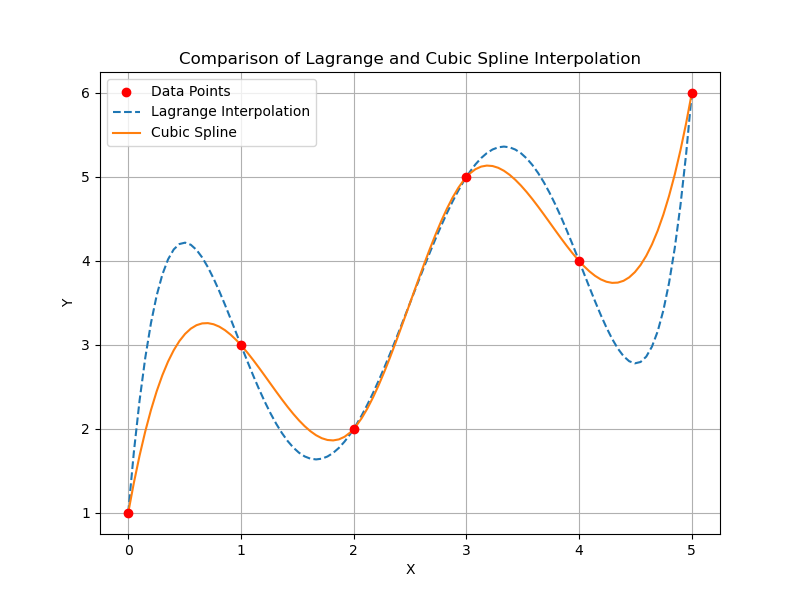
\includegraphics[width=0.7\textwidth]{problem-1/Figure_1.png}
		\caption{مقایسۀ درونیابی \lr{Lagrange} و \lr{Cubic Spline}}
	\end{figure}
	
	\newpage
	
	\section*{سوال ۲}
	در این بخش، داده‌های ذخیره‌شده در فایل \lr{data.xlsx} خوانده شدند و سپس رفتار سه الگوریتم مختلف از نظر زمان اجرا بررسی شد. هدف اصلی این بود که روند افزایش زمان اجرا با رشد حجم داده‌ها تحلیل شود.
	
	فایل داده شامل ستون‌های مربوط به اندازه داده و زمان اجرای سه الگوریتم \lr{Alg.1}، \lr{Alg.2} و \lr{Alg.3} بود. این داده‌ها با استفاده از کتابخانۀ \lr{pandas} بارگذاری شدند و سپس با استفاده از \lr{matplotlib} نمودارهای مناسب برای تحلیل آن‌ها ترسیم شد.
	
	ابتدا داده‌ها در قالب یک نمودار خطی با مقیاس معمولی رسم شدند. این نمودار نشان می‌دهد که با افزایش اندازه داده از \lr{100KB} تا \lr{600KB}، هر سه الگوریتم رشد زمانی دارند، اما شیب رشد آن‌ها متفاوت است. \lr{Alg.1} کمترین رشد را دارد، در حالی که \lr{Alg.3} سریع‌ترین افزایش را نشان می‌دهد.
	
	برای درک بهتر رفتار الگوریتم‌ها، نمودار دوم با مقیاس لگاریتمی (\lr{Log Scale}) رسم شد. در این نمودار نیز مشخص است که \lr{Alg.1} از نظر زمان اجرا بسیار بهینه‌تر از دو الگوریتم دیگر است.
	
	در مرحلۀ بعد، یک دادۀ جدید مربوط به \lr{700KB} به دیتافریم اضافه شد. مقدار افزوده‌شده برای این سطر به صورت زیر بود:
	\[
	\text{\lr{Alg.1}}=80,\quad \text{\lr{Alg.2}}=320,\quad \text{\lr{Alg.3}}=700
	\]
	افزودن این داده باعث شد روند کلی مقایسه کامل‌تر شود و پیش‌بینی رفتار الگوریتم‌ها در اندازه‌های بزرگ‌تر نیز امکان‌پذیر باشد.
	
	علاوه بر نمودارهای خطی، یک نمودار میله‌ای (\lr{Bar Chart}) نیز برای مجموع زمان اجرای هر الگوریتم رسم شد. مجموع زمان اجرای \lr{Alg.1} کمترین مقدار را دارد، در حالی که \lr{Alg.3} بیشترین زمان کل را مصرف می‌کند. بر اساس محاسبات انجام‌شده:
	\begin{itemize}
		\item مجموع زمان اجرای \lr{Alg.1} برابر با \lr{375} و میانگین آن \lr{62.50} است.
		\item مجموع زمان اجرای \lr{Alg.2} برابر با \lr{1500} و میانگین آن \lr{250.00} است.
		\item مجموع زمان اجرای \lr{Alg.3} برابر با \lr{2100} و میانگین آن \lr{350.00} است.
	\end{itemize}
	
	همچنین میانگین زمان اجرای \lr{Alg.2} برای داده‌های \lr{100KB} تا \lr{600KB} محاسبه شد و مقدار آن برابر با \textbf{\lr{250.00}} به دست آمد.
	
	\begin{figure}[ht]
		\centering
		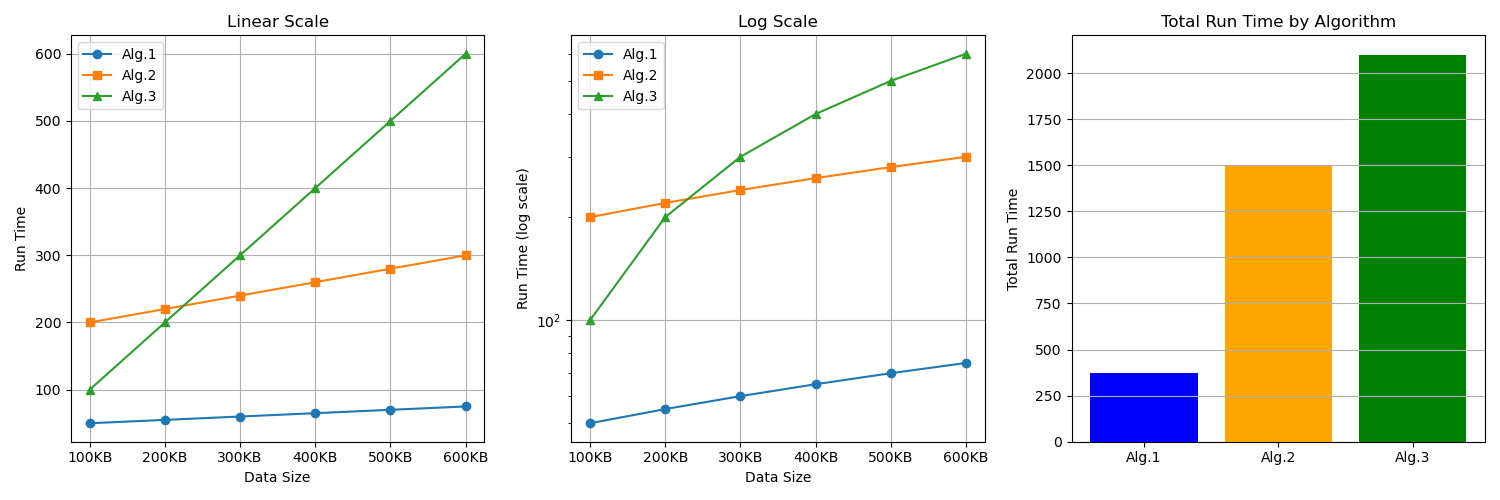
\includegraphics[width=1\textwidth]{problem-2/Figure_1.png}
		\caption{تحلیل زمان اجرای الگوریتم‌های \lr{1}، \lr{2} و \lr{3}}
	\end{figure}
	
	\section*{سوال ۳}
	در این بخش، محاسبۀ عددی انتگرال تابع $ f(x)=e^{x^2} $ در بازۀ $[0,1]$ بررسی شد. از آنجا که انتگرال این تابع در فرم تحلیلی ساده قابل محاسبه نیست، استفاده از روش‌های عددی ضروری است.
	
	ابتدا از \textbf{روش ذوزنقه‌ای} (\lr{Trapezoidal Rule}) استفاده شد. سپس از \textbf{روش سیمپسون} (\lr{Simpson's Rule}) استفاده شد که به جای خطوط مستقیم، از چندجمله‌ای‌های درجه دو برای تقریب تابع بهره می‌برد.
	
	نتایج محاسبه‌شده نشان دادند که:
	\begin{itemize}
		\item مقدار تقریبی انتگرال با روش ذوزنقه‌ای برابر است با \textbf{\lr{1.462697}}
		\item مقدار تقریبی انتگرال با روش سیمپسون برابر است با \textbf{\lr{1.462652}}
	\end{itemize}
	
	در ادامه، \textbf{کوادراتور گوسی ۵ نقطه‌ای} (\lr{Gaussian Quadrature}) نیز به کار گرفته شد. در این پروژه، نتیجه به‌دست‌آمده از روش گوسی برابر با \textbf{\lr{1.462652}} بود که کاملاً با نتیجه روش سیمپسون منطبق است. این هم‌خوانی میان روش سیمپسون و کوادراتور گوسی نشان می‌دهد که هر دو روش تقریب بسیار دقیقی برای این تابع ارائه می‌دهند.
	
	
\end{document}
